%% -*- coding:sjis -*-
%%
%% 2013-07-19, Koichi Murase, 入力
%%
\def\kB{k_{\mathrm{B}}}
\begin{question}{第1問}{村瀬}
量子論における軌道角運動量$\bm{l}$は古典論と同様に座標$\bm{r}$と運動量$\bm{p}$のベクトル積で与えられ
る。すなわち$\bm l=\bm r \times \bm p$である。ここで、それぞれのベクトルの成分は
$\bm r=(x,y,z),\,\bm p=(p_x,p_y,p_z),\,\bm l=(l_x,l_y,l_z)$である。
以下の設問に答えよ。ただし、$\hbar = \frac{h}{2\pi}$ ($h$はプランク定数)
を用いよ。
\begin{enumerate}
\item $l_z$と$x,y,z$との間の交換関係を求めよ。
\item $l_z$と$p_x,p_y,p_z$との間の交換関係を求めよ。
\item\ilabel{Q1.3}
  $l_a$と$l_b$との間の交換関係を求めよ。ただし、$a,b=x,y,z$である。
\end{enumerate}

量子論では、軌道角運動量$\bm l$を拡張して設問\iref{Q1.3}の交換関係を満たす演算子を角運動量$\bm J$と呼ぶ。
以下では、角運動量$\bm J$のみが力学変数である力学系を考える。ここで、変数$A$を$A=J_x-iJ_y$, 
変数$B$を$B=J_x^2+J_y^2+J_z^2$と定義する。次の設問に答えよ。
\begin{enumerate}
\setcounter{enumi}{3}
\item $A^\dag A$および$AA^\dag$を$B$と$J_z$を用いて書け。ただし、$A^\dag$は$A$の複素共役演算子である。
\item $B$は演算子ではなくただの数であることを示せ。
\end{enumerate}
$J_z$は固有値を持つと考えて、その固有値を$\Theta_z$および固有状態を$|\Theta_z\rangle$とする。次の設問に答
えよ。
\begin{enumerate}
\setcounter{enumi}{5}
\item $A|\Theta_z\rangle\neq 0$ ならば $A|\Theta_z\rangle$も$J_z$の固有状態であることを示せ。また、その固有値を求めよ。
\item $\langle\Theta_z|A^\dag A|\Theta_z\rangle\ge0$と
  $\langle\Theta_z|A A^\dag|\Theta_z\rangle\ge0$を用いて、
  $-m\le\Theta_z\le m$を証明せよ。ただし、
  $m=\sqrt{B+\frac14\hbar^2-\frac12\hbar}$である。
\item 以上の結果を用いて、$m$が$\hbar$の整数倍であるかまたは半整数倍であることを示せ。
\end{enumerate}
\end{question}

\begin{question}{第2問}{村瀬}
スピン$1/2$の粒子が大きさ$H$の磁場の下におかれると、ゼーマン効果によって、そのエネル
ギー準位は$-\mu H,+\mu H$($\mu$は正の定数)に分裂する。このような粒子$N$個が大きさ$H$の一様
な磁場の下におかれ、温度$T$に保たれている系を考え、これをカノニカル分布によって取り扱
う。最初は粒子間に相互作用がないとして、以下の設問に答えよ。ただし、$\beta=(\kB T)^{-1}$ ($\kB$
はボルツマン定数)を用いてもよい。
\begin{enumerate}
\item
  この系の自由エネルギー$F$を求めよ。
\item
  磁場に平行方向の磁化$M$と、$H\to0$での磁化率$\chi$を求めよ。ただし磁化は$M=-\partial F/\partial H$、
  磁化率は$\chi=\partial M/\partial H$で定義される。
\end{enumerate}
次に、$N$個の粒子が2個ずつ$N/2$組の対になり、対を組んだ粒子間にはそれぞれのスピンの内
積に比例する相互作用が働く場合を考える。異なる対に含まれる粒子間には相互作用が働かな
いとする。磁場の方向を$z$方向とすれば、一つの対のハミルトニアンは、対に含まれる2粒子
のスピン演算子$\bm{s}_1,\bm{s}_2$とその$z$成分$s_{1z},s_{2z}$を用いて、
\begin{align*}
  \mathcal{H} = V\bm s_1\cdot \bm s_2 -2\mu(s_{1z}+s_{2z})H
\end{align*}
と書くことができる。$V$は相互作用の大きさと符号を表すパラメータである。このとき以下の
設問に答えよ。
\begin{enumerate}
\setcounter{enumi}{2}
\item ハミルトニアン$\mathcal H$のエネルギー固有値を求めよ。
\item $N/2$組の対からなる系全体の自由エネルギー$F$を求めよ。
\item\ilabel{Q2.5}
  磁場に平行方向の磁化$M$と、$H\to0$での磁化率$\chi$を求めよ。
\item
  設問\iref{Q2.5}で求めた磁化率の低温極限($\kB T/|V|\ll1$)での振舞いを調べ、それが$V$の符号に
  よって定性的に異なる理由を簡単に説明せよ。
\end{enumerate}
\end{question}

\begin{question}{第3問}{村瀬}
質量$m_1$の太陽と質量$m_2$の地球がお互いの重力によってケプラー運動しているものとする。簡
単のために以下では軌道の離心率は無視して円運動の場合のみを考える。それらの公転面上で
太陽と地球の重心を原点とする2次元座標系として、慣性系$S$と、太陽と地球が常に$x$軸上の
点$P_1$と点$P_2$に位置するような回転系$S'$を考える(図1参照)。太陽と地球の距離を$a$とすれ
ば、$P_1$と$P_2$の座標はそれぞれ$(-\mu_2a,0)$、$(\mu_1a,0)$で与えられる。ただし、
\begin{align}
  \mu\equiv\frac{m_1}{m_1+m_2},\quad
  \mu_2\equiv\frac{m_2}{m_1+m_2} \ilabel{eq:Q3.1}
\end{align}
である。また、この回転系の角速度$\omega$はケプラーの第3法則より、
\begin{align}
  G(m_1+m_2)=\omega^2a^3 \ilabel{eq:Q3.2}
\end{align}
を満たす($G$はニュートンの重力定数)。
\begin{center}
  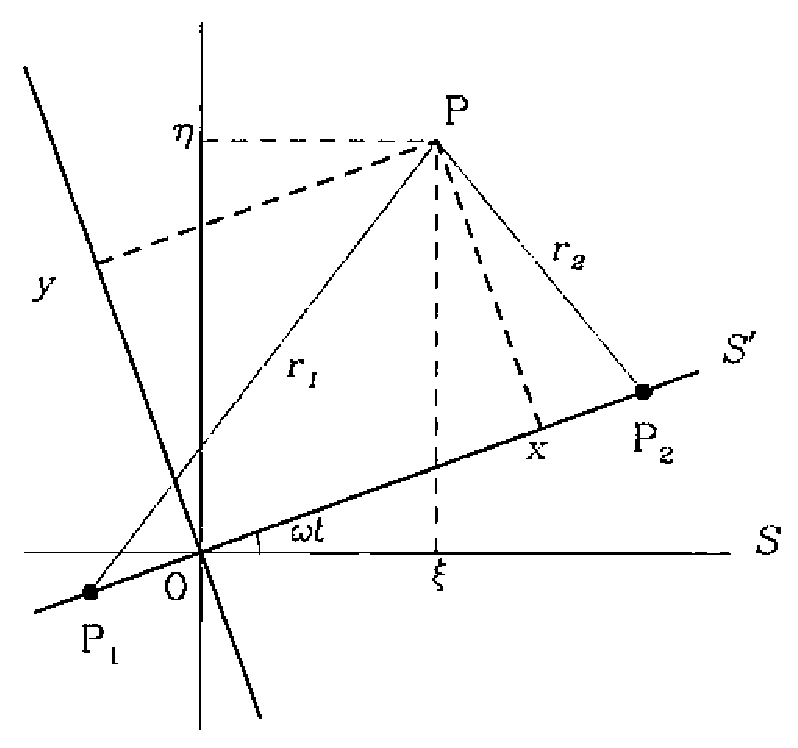
\includegraphics[width=0.6\textwidth]{2006physQ3_1r.eps}\\図1
\end{center}
\begin{enumerate}
\item\ilabel{Q3.1}
  この平面上の任意の点を$P$としたとき、$S$系における$P$の成分$(\xi,\eta)$を$S'$系での成分
  $(x,y)$で表わせ。
\item
  $S'$系からみて$(x,y)$の位置にある質量$m$の質点を考える。$m$は$m_1$および$m_2$に比べて
  十分小さく、この質点は太陽と地球のケプラー運動には影響を与えないとした時、設問\iref{Q3.1}
  の結果からこの質点に対するラグランジアンが
  \begin{align}
    \mathcal{L}=\frac m2(\dot x^2 + \dot y^2)
    + \frac{m\omega^2}2 (x^2+y^2) + m\omega(x\dot y-\dot x y)
    + Gm\left(\frac{m_1}{r_1}+\frac{m_2}{r_2}\right) \ilabel{eq:Q3.3}
  \end{align}
  となることを示せ。ただし、
  \begin{align}
    r_1\equiv\sqrt{(x+\mu_2a)^2+y^2},\quad
    r_2\equiv\sqrt{(x-\mu_1a)^2+y^2} \ilabel{eq:Q3.4}
  \end{align}
  である。
\item
  この質点の$S'$系における運動方程式の$x$成分および$y$成分を書き下せ。
\item
  $S'$系から見たとき、この質点の加速度と速度がともに0となるような特別な点
  $(\ddot x=\ddot y= \dot x = \dot y=0)$はラグランジュ点と呼ばれ、全部で5つあることが知られている。運動方程
  式の$y$成分を考えることで、ラグランジュ点は
  \begin{align}
    \mu_1\left(\frac{a}{r_1}\right)^3
    + \mu_2\left(\frac{a}{r_2}\right)^3 = 1 \ilabel{eq:Q3.5}
  \end{align}
  あるいは
  \begin{align}
    y=0 \ilabel{eq:Q3.6}
  \end{align}
  のいずれかを満たすことを示せ。

\item
  式\ieqref{eq:Q3.6}を満たす$S'$系の$x$軸上にあるラグランジュ点は、図2に示されているように、$P_1$
  と$P_2$の外側に一つずつ、および$P_1$と$P_2$の中間に一つ、合わせて3個存在することが知
  られている。特に地球からみてちょうど太陽の反対側にある$L_2$点は、天文観測衛星に適
  した位置である。この$L_2$点と$P_2$との距離を$r_2$として運動方程式の$x$成分を考えれば、
  $\mu_2/\mu_1$が$u\equiv r_2/a$の関数として
  \begin{align}
    \frac{\mu_2}{\mu_1} = \frac{3u^3}{(1+u)^2}\frac{1+u+u^2/3}{1-u^3} \ilabel{eq:Q3.7}
  \end{align}
  と書けることを示せ。変形の際、$\mu_1+\mu_2=1$であることに注意せよ。
  \begin{center}
    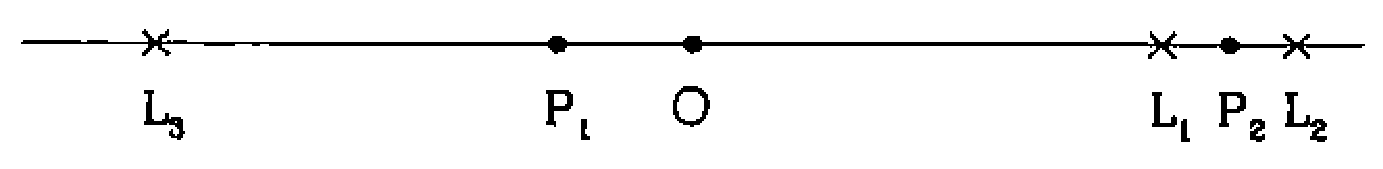
\includegraphics[width=0.75\textwidth]{2006physQ3_2r.eps}\\図2
  \end{center}
\item
  式\ieqref{eq:Q3.7}から、$\mu_2/\mu_1\ll1$の場合$u\ll1$となることがわかる。この場合、$L_2$点の位置$u$を
  $\mu_2/\mu_1$の最低次で求めよ。特に、太陽と地球の系($\mu_2/\mu_1\approx3\times10^{-6}$、$a=1.5\times10^{11}$m)
  の場合、地球と$L_2$点までの距離の値を近似的に求めよ。
\end{enumerate}
\end{question}

\begin{question}{第4問}{村瀬}
中性子と原子核との弾性散乱を利用して中性子を検出したい。これに関連した以下の設問に答
えよ。ただし運動はすべて非相対論的に扱えるものとし、必要に応じて、中性子質量$=$陽子質
竜$=$1000 MeV/$c^2$($c$は光速)、質量数$A$の原子核の質量=1000$A$MeV/$c^2$を用いよ。
\begin{enumerate}
\item
  運動エネルギー$T$rの中性子が、静止した質量数$A$の原子核と弾性散乱する際、原子核に
  与えられる反跳エネルギーの最大値$E_\mathrm{max}$を求めよ。また$E_\mathrm{max}$は$A=1$、すなわち陽子
  と散乱する場合に最大となることを示せ。

\item
  中性子-陽子の弾性散乱における陽子の反跳エネルギー分布$dW/dE$を、以下の手順で求
  めよ。ここで$dW$は陽子の反跳エネルギーが$E$と$E+dE$との間にある確率である。
  \begin{enumerate}
  \item\ilabel{Q4.2a}
    陽子の反跳エネルギー$E$を、中性子のエネルギー$T$と重心系での散乱角$\theta^*$(図1参
    照)で表せ。
  \item
    散乱は重心系において等方的、すなわち$d\sigma/d\Omega^*=一定$であるとする。ただし$\sigma$は
    散乱断面積、$\Omega^*$は重心系での立体角である。設問\iref{Q4.2a}で求めた$E$と$\theta^*$の関係を利
    用して$dW/dE$を求め、その概略を図示せよ。
  \end{enumerate}
\end{enumerate}

以下では、中性子検出器として、プラスチック・シンチレーター(密度1g/cm$^3$、元素組成が
C:H$=$1:1である蛍光物質)と光電子増倍管を組み合わせたものを用いる場合を考える。た
だし、中性子と炭素の衝突による効果は無視でき、また、検出器は反跳陽子を100\%の効率で
検出できるものとする。次の設問に答えよ。

\begin{enumerate}
\setcounter{enumi}{2}
\item
  この検出器に中性子が入射してから光電子増倍管から電気信号が出るまでの過程を200
  字以内で記述せよ。

\item
  シンチレーター中での中性子の平均自由行程$\lambda$を、中性子と陽子の弾性散乱断面積$\sigma$と
  単位体積あたりの水素原子数$n$を用いて表せ。

\item
  シンチレーターの厚さが$x$の場合の中性子検出効率(検出器が厚い場合にも適用できる一般式
  )を、$\lambda$と$x$を用いて表せ。

\item
  図2に示す中性子と陽子の弾性散乱断面積のグラフを用いて、厚さ10cmのプラスチッ
  ク・シンチレーターの、運動エネルギー20MeVの中性子に対する検出効率を精度一桁
  で概算せよ。必要に応じてアボガドロ数$N_A=6\times10^{23}$を用いよ。
\end{enumerate}
\begin{center}
  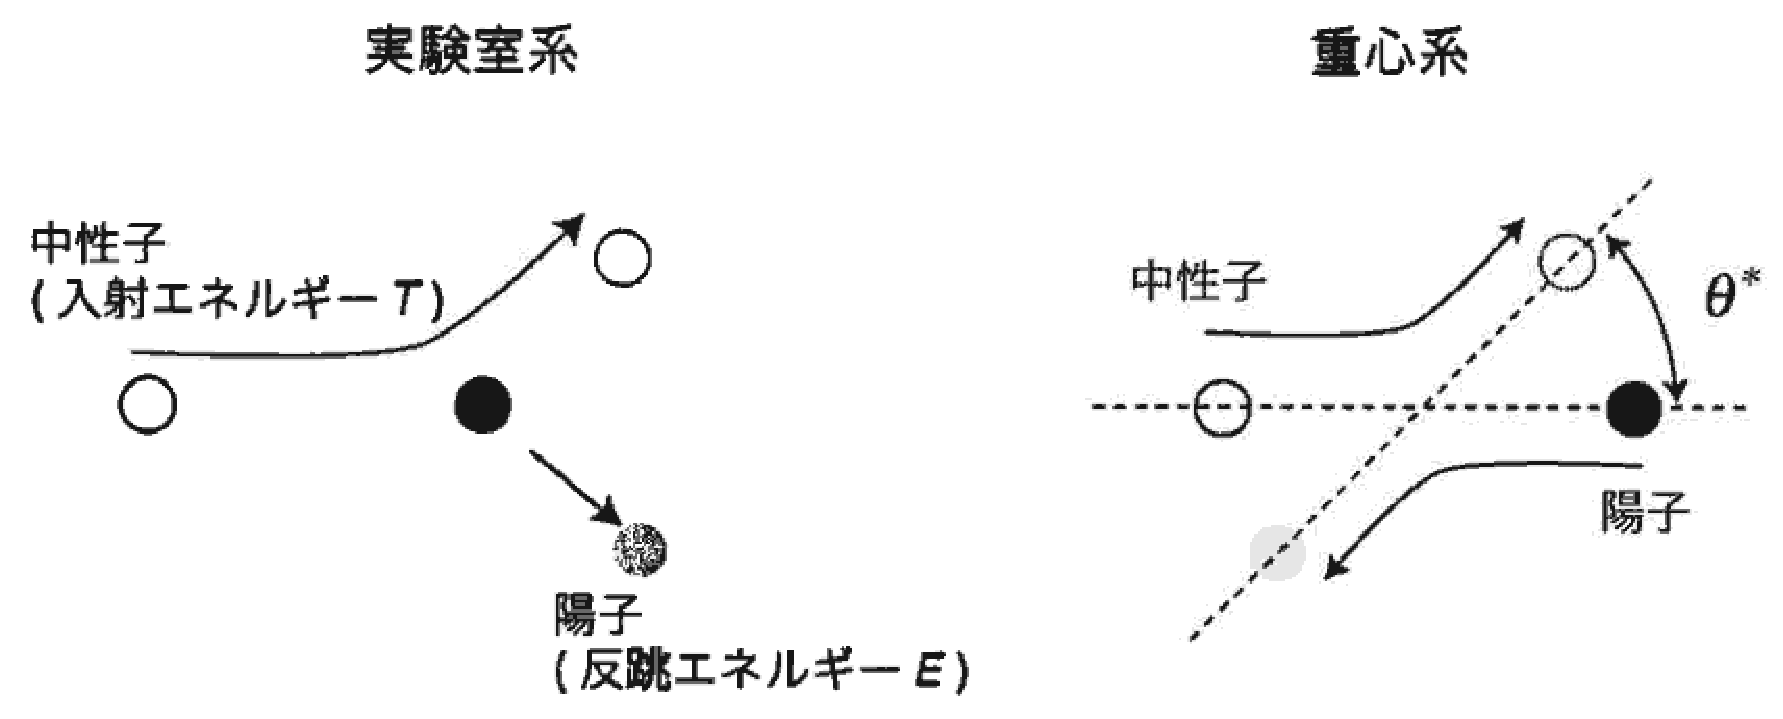
\includegraphics[width=0.8\textwidth]{2006physQ4_1r.eps}\\図1
\end{center}
\begin{center}
  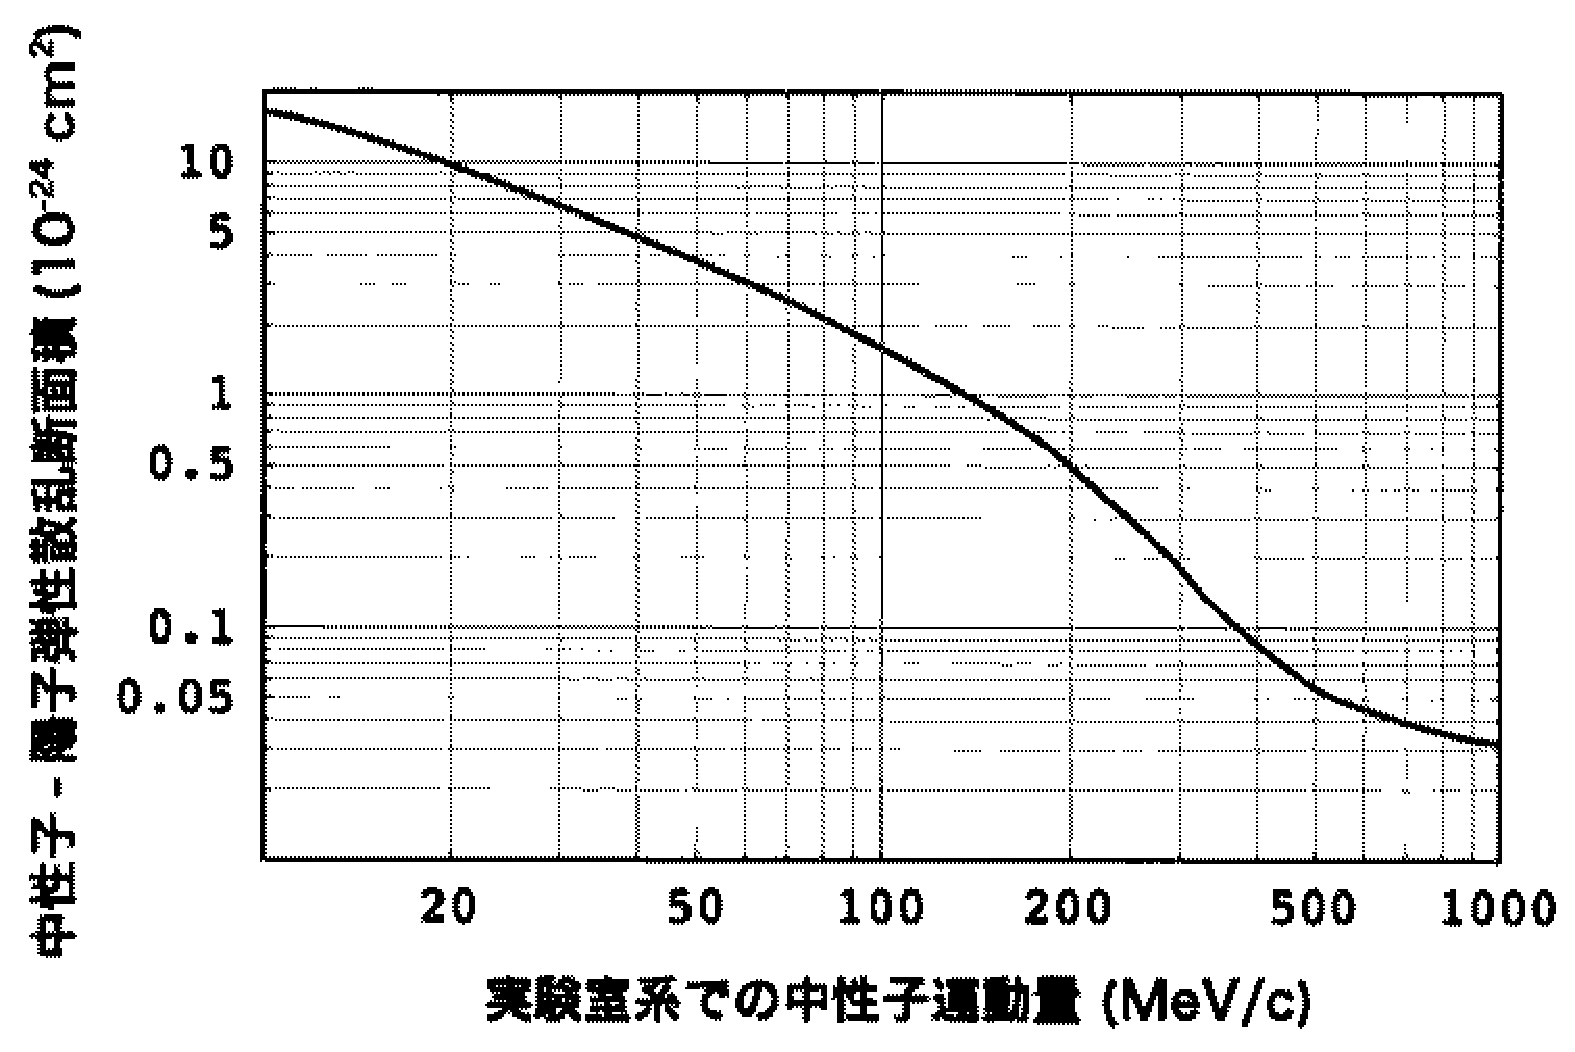
\includegraphics[width=0.8\textwidth]{2006physQ4_2r.eps}\\図2
\end{center}
\end{question}

\begin{question}{第5問}{村瀬}
比熱測定は物質のエントロピーや内部エネルギー、さらには相転移現象について有用な情報が
得られる実験手段である。低温での比熱測定に関連して以下の設問に答えよ。
\begin{enumerate}
\item
  一般に固体の比熱は図1に示すような装置を用いて測定できる。ヒーターおよび抵抗温
  度計が取り付けられた基板上に試料を乗せ、ヒーターで一定の熱量を加えたときの温度
  上昇から比熱が求まる。この測定を精度良く行うために実験上注意すべき点を200字以
  内で述べよ。
  \begin{center}
    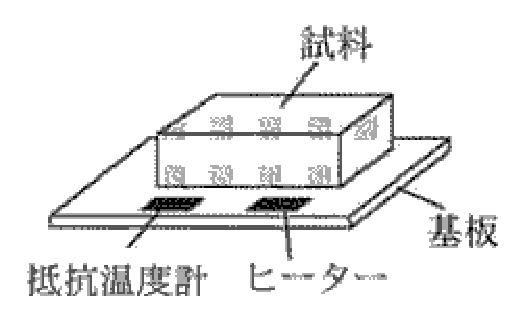
\includegraphics[width=0.25\textwidth]{2006physQ5_1r.eps}\\図1
  \end{center}
\item
  比熱$C(T)$を用いてエントロピー$S(T)$および内部エネルギー$U(T)$を表せ。ただし、$T=0$
  での内部エネルギー$U(0)$を用い、また$S(0)=0$とせよ。
\item
  図1の装置を用いてアルミニウムの1モル当たりの比熱$C$を温度範囲 1.22K$\le T \le4$K
  で測定した結果を、縦軸に$C/T$、横軸に$T^2$をとって図2に$\circ$印で示す。この図から$C(T)$
  には格子振動を起源とする$T^3$に依存する項の他に、より主要な寄与があることがわか
  る。その温度依存性と係数、およびその起源を答えよ。
\end{enumerate}
\begin{center}
  \begin{minipage}[t]{0.45\textwidth}
    \begin{center}
      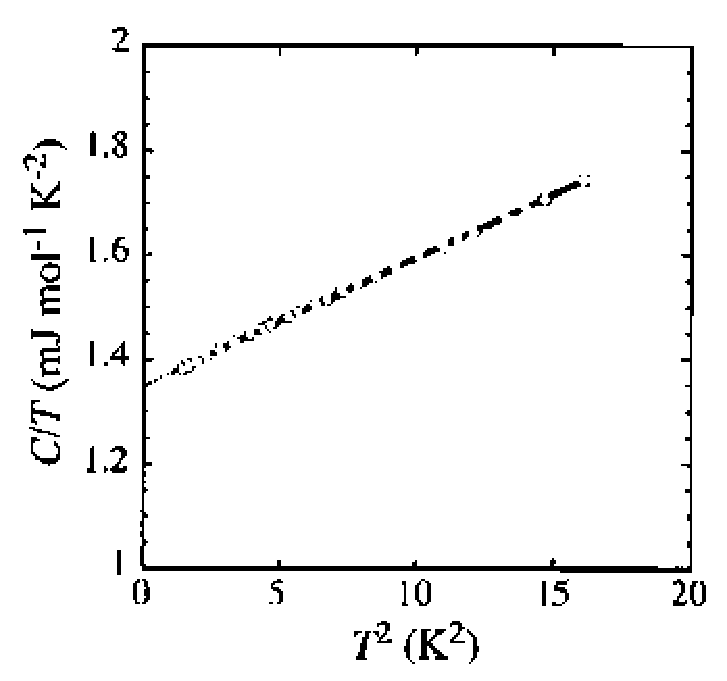
\includegraphics[width=0.8\textwidth]{2006physQ5_2r.eps}\\図2
    \end{center}
  \end{minipage}
  \begin{minipage}[t]{0.45\textwidth}
    \begin{center}
      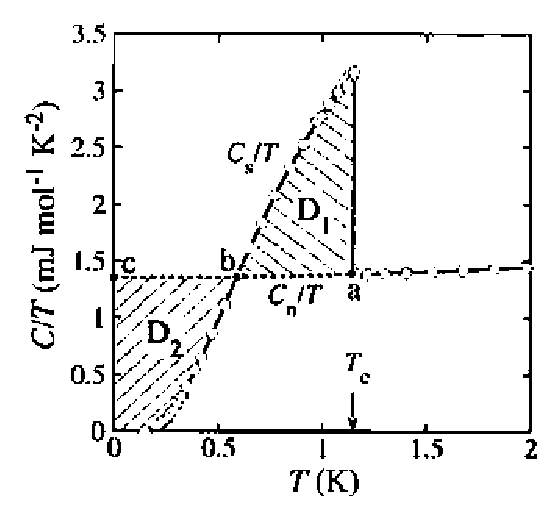
\includegraphics[width=0.8\textwidth]{2006physQ5_3r.eps}\\図3
    \end{center}
  \end{minipage}
\end{center}
アルミニウムの比熱をより低温の0.2Kまで測定した結果について縦軸に$C/T$、横軸に$T$を
とって描いたものを図3に示す。この図の点線(a-b-c)は図2のデータを低温まで外挿したも
ので、通常の金属で期待される振舞いである(正常状態と呼ぶ)。実際の測定データはこの延
長線上には乗らず、転移温度$T_\mathrm{c}=1.16$Kで2次相転移(超伝導転移)による飛びを示した。こ
こで $C_\mathrm{s}$、$C_\mathrm{n}$はそれぞれ超伝導状態および正常状態における比熱を表す。
\begin{enumerate}
\setcounter{enumi}{3}
\item
  $T_\mathrm{c}$における相転移が2次相転移であることに注意して、図3の領域D$_1$と領域D$_2$の面積
  が等しくなることを示せ。
\end{enumerate}
超伝導状態にあるアルミニウムに大きさ$H$の磁場をかけると、ある磁場で超伝導が壊れて正常
状態に1次相転移する。このときの磁場を臨界磁場$H_\mathrm{c}$と呼ぶ。次にこの相転移を熱力学的に考
察しよう。磁場中における、正常状態および超伝導状態の自由エネルギー$G_\mathrm{n}(T,H)$、$G_\mathrm{s}(T,H)$
は次式で与えられる。
\begin{align}
  G_{\mathrm{n},\mathrm{s}}(T,H)
  = G_{\mathrm{n},\mathrm{s}}(T,0) - V\int_0^H BdH \ilabel{eq:Q5.8}
\end{align}
ここで$V$はアルミニウムのモル体積、$B$は試料内の磁束密度を表し一様とする。そして正常状
態では$B=\mu_0H$($\mu_0=4\pi\times10^{-7}$H/m)、超伝導状態では$B=0$であるとする。$G_\mathrm{n}(T,0)$、
$G_\mathrm{s}(T,0)$は$G=U-TS$の関係式を使って比熱の測定データから求めることができる。その温
度依存性を示したものが図4である。ただし$G_\mathrm{n}(0,0)=0$とした。
\begin{enumerate}
\setcounter{enumi}{4}
\item
  $G_\mathrm{n}(T,H)$および$G_\mathrm{s}(T,H)$の磁場依存性を表す式を示せ。また図4を参考に一定磁場$H$
  のもとでの$G_\mathrm{n}$と$G_\mathrm{s}$の温度依存性を図示して、この相転移が1次転移である理由を述べ
  よ。ただし$G_\mathrm{n}(0,H)>G_\mathrm{s}(0,H)$が成り立つ磁場範囲について答えよ。
\item
  $T=0$におけるアルミニウムの臨界磁束密度$B_\mathrm{c}(0)=\mu_0H_\mathrm{c}(0)$を図4のデータをもとに
  有効数字1桁で求めよ。ただし、アルミニウムのモル体積は10cm$^3$/molとする。
\item
  この様にして求めたアルミニウムの臨界磁場の温度依存性を図5に示す。$T/T_\mathrm{c}\ll1$で
  は$H_\mathrm{c}(T)=H_\mathrm{c}(0)(1-aT^2)$($a$は定数)となることが知られている。正常状態の$C/T$の
  $T=0$への外挿値を$\gamma$、また$\delta=G_\mathrm{n}(0,0)-G_\mathrm{s}(0,0)$として、$a$を$\gamma$および$\delta$を用いて
  表せ。
\end{enumerate}
\begin{center}
  \begin{minipage}[t]{0.55\textwidth}
    \begin{center}
      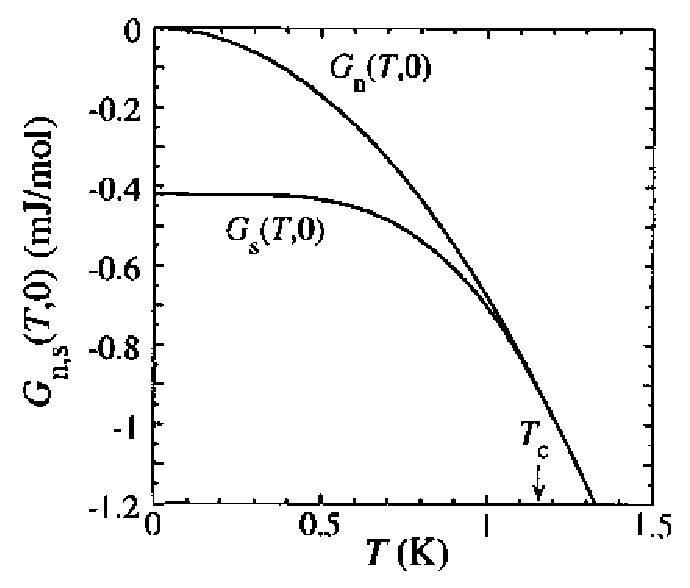
\includegraphics[width=0.8\textwidth]{2006physQ5_4r.eps}\\図4
    \end{center}
  \end{minipage}
  \begin{minipage}[t]{0.35\textwidth}
    \begin{center}
      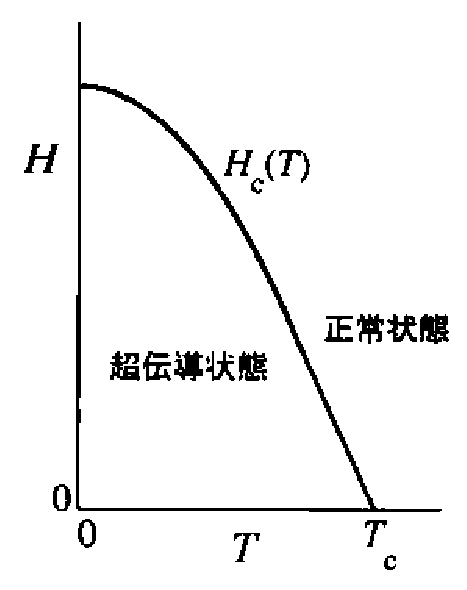
\includegraphics[width=0.8\textwidth]{2006physQ5_5r.eps}\\図5
    \end{center}
  \end{minipage}
\end{center}
\end{question}

\begin{question}{第6問}{村瀬}
図1は、水素原子の主量子数$n=2$のエネルギー準位構造を示している。$2P_{3/2}(j=3/2)$と
$2S_{1/2}(j=1/2)$とのエネルギー差を$h\nu_1$、$2S_{1/2}(j=1/2)$と$2P_{1/2}(j=1/2)$とのエネルギー差
を$h\nu_2$とする。ただし、$h$はプランク定数、$j$は電子の軌道角運動量$\bm{l}$とスピン角運動量$\bm{s}$を合
成した角運動量$\bm{j}=\bm{l}+\bm{s}$の大きさを$\hbar$を単位として表した量子数である。
\begin{center}
  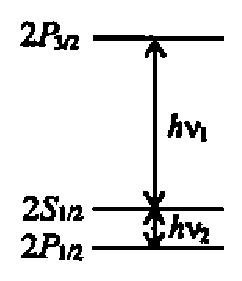
\includegraphics[width=0.15\textwidth]{2006physQ6_1r.eps}\\図1
\end{center}
図2(a)は、このエネルギー差$h\nu_1$、$h\nu_2$を精密に測定するための実験装置である。$1S_{1/2}$にある
水素原子を、電子線との衝突により$2S_{1/2}$へ励起する。$2S_{1/2}$は寿命が$2P_{1/2}$、$2P_{3/2}$に比べ著
しく長いため、$1S_{1/2}$に遷移する前に金属板に衝突する。そのとき放出される電子を対向電極
(正極)で捕らえることにより、$2S_{1/2}$にある原子数を検流計の電流値として観測することがで
きる。導波管内で原子に照射するマイクロ波の周波数が、例えば$\nu_1$に一致(共鳴)すると、図
2(b)に示すように$2P_{3/2}$への遷移が起き、この準位からは速やかに$1S_{1/2}$へ自発放射により遷
移するため、金属板から電子が放出されず検流計の電流値は減少する。
\begin{enumerate}
\item
  この実験装置では、電子線発生器のグリッド、アノードは接地されている。フィラメント
  (カソード)の電位は何Vに設定するのが適当か、理由と共に答えよ(ヒント:水素原子
  のイオン化エネルギーは13.6eV)。
\item
  一般に、原子が自発放射によって遷移する確率は、始状態と終状態の間の電気双極子モー
  メントの大きさの2乗に比例する。$2S_{1/2}$の寿命が$2P_{1/2}$、$2P_{3/2}$に比べ著しく長い理由
  を簡潔に述べよ。
\end{enumerate}
\begin{center}
  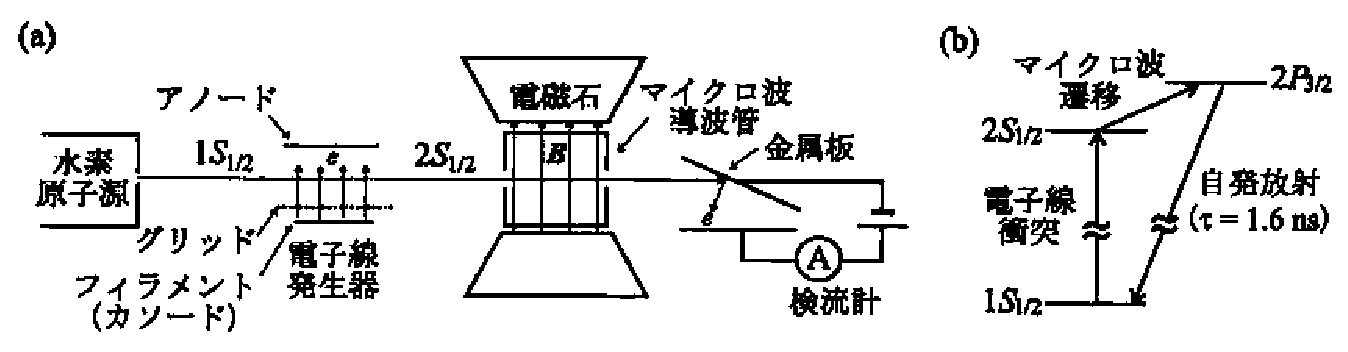
\includegraphics[width=0.8\textwidth]{2006physQ6_2r.eps}\\図2
\end{center}
電磁石を用いて導波管内に外部磁場を印加すると、$2S_{1/2}$、$2P_{3/2}$の磁気副準位のエネルギーは
ゼーマンシフトする。外部磁場と水素原子との相互作用(ゼーマンエネルギー)を表すハミル
トニアンは、磁場の向きを$z$軸にとれば、
\begin{align*}
  \mathcal{H}_z = \frac{\mu_B}{\hbar}(l_x + 2s_z) B
\end{align*}
と表される。ただし、$\mu_B$はボーア磁子、$B$は磁場(磁束密度)の大きさである。図3(a)に
$2S_{1/2}$, $2P_{3/2}$の磁気副準位のゼーマンシフトの様子を示す(縦軸の目盛は省略されている)。図
中の$m$は角運動量$\bm j$の磁気量子数を表す。
\begin{enumerate}
\setcounter{enumi}{2}
\item\ilabel{Q6.3}
  マイクロ波遷移$\alpha(2S_{1/2},m=1/2)\to\mathrm{a}(2P_{3/2},m=1/2)$の共鳴周波数のゼーマン効果に
  よる変化量を$\Delta\nu$とする。$\Delta\nu$の磁場依存性を$\mu_B, B$を用いて表せ。
\item
  図3(b)は、マイクロ波周波数11.5GHzにおいて、磁場の大きさを変化させながら検流
  計の電流値の減少量を測定して得られたマイクロ波遷移$\alpha\to\mathrm{a}$の共鳴曲線である。この
  実験結果、および設問\iref{Q6.3}の結果を用いて、$\nu_1$の値を有効数字2桁で計算せよ(ヒント:
  $\mu_B/h\approx$14GHz/T)。
\item
  $2P_{3/2}$準位の寿命($\tau=1.6$ns)で決まるマイクロ波遷移$\alpha\to\mathrm{a}$の共鳴曲線の線幅を有効
  数字2桁で計算せよ。図3(b)で観測された共鳴曲線の線幅は、$2P_{3/2}$準位の寿命で決ま
  る線幅よりも広い。その要因として考えられるものを挙げよ。
\end{enumerate}
\begin{center}
  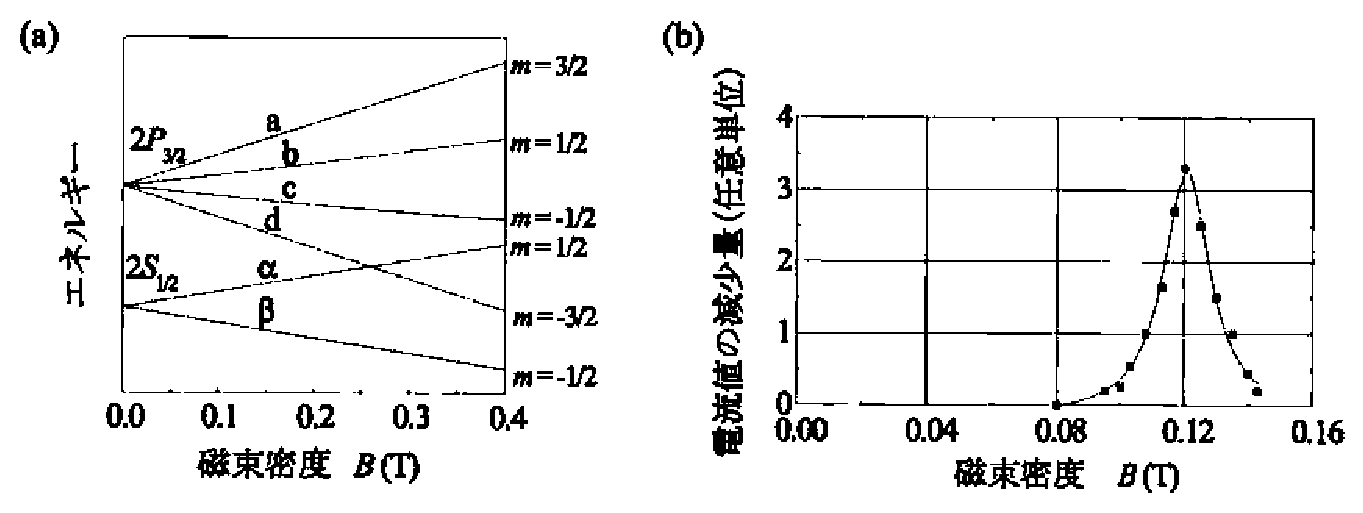
\includegraphics[width=0.8\textwidth]{2006physQ6_3r.eps}\\図3
\end{center}
1947年、LambとRetherfordは図2(8)の実験装置を用いて、$\nu_1$と同時に$\nu_2$の値も精密に測定
し、Diracの相対論的電子諭では縮退すると予言されていた$2S_{1/2}$および$2P_{1/2}$準位が、実際に
は分裂していることを確認した。この分裂はラムシフトと呼ばれている。
\begin{enumerate}
\setcounter{enumi}{5}
\item
  ラムシフトは、電磁場の真空揺らぎ(零点振動)によって点電荷が実効的に有限な広が
  りを持つと考えることによって定性的に説明できる。この考え方を用いて、ラムシフト
  により$2S_{1/2}$のエネルギーが$2P_{1/2}$よりわずかに高くなる理由を述べよ。
\end{enumerate}
\end{question}
